\documentclass[11pt,a4paper]{article}
% Standalone English report. Compile from the report/ directory.
\usepackage[T1]{fontenc}
\usepackage[utf8]{inputenc}
\usepackage[english]{babel}
\usepackage[a4paper,margin=21mm]{geometry}
\usepackage{lmodern}
\usepackage{microtype}
\usepackage{amsmath,amssymb}
\usepackage{graphicx}
\usepackage[pdftex]{lscape}
\usepackage{booktabs,tabularx,array}
\usepackage{tikz}
\usetikzlibrary{arrows.meta,positioning}
\usepackage[hidelinks]{hyperref}
\setlength{\parindent}{0pt}
\setlength{\parskip}{3pt}
\setlength{\emergencystretch}{2em}
\renewcommand{\arraystretch}{1.15}
\newcommand{\code}[1]{\texttt{\detokenize{#1}}}
% Derived only from saved CSV/JSON outputs; values rounded for display.
\newcommand{\ScanBatches}{14\,344}
\newcommand{\ScanEdges}{14\,605\,144}
\newcommand{\ScanMembers}{246}
\newcommand{\ScanNonMembers}{14\,098}
\newcommand{\ScanMin}{0.003385}
\newcommand{\ScanMax}{1.785713}
\newcommand{\ScanMean}{0.347405}
\newcommand{\ScanMedian}{0.412648}
\newcommand{\ScanLowerQuartile}{0.003737}
\newcommand{\ScanUpperQuartile}{0.694921}
\newcommand{\ScanPercentileNinetyFive}{0.699984}
\newcommand{\ScanPercentileNinetyNine}{0.977328}
\newcommand{\ScanWithMean}{0.719045}
\newcommand{\ScanWithMedian}{0.696006}
\newcommand{\ScanWithoutMean}{0.340920}
\newcommand{\ScanWithoutMedian}{0.370385}
\newcommand{\InitialReference}{0.829613}
\newcommand{\InitialOriginal}{0.717195}
\newcommand{\InitialSum}{-0.112418}
\newcommand{\HighMemberReference}{2.076339}
\newcommand{\HighMemberOriginal}{1.785713}
\newcommand{\HighMemberSum}{-0.290626}
\newcommand{\HighNoMemberReference}{1.832905}
\newcommand{\HighNoMemberOriginal}{1.782047}
\newcommand{\HighNoMemberSum}{-0.050858}
\newcommand{\LowMemberReference}{0.064803}
\newcommand{\LowMemberOriginal}{0.047847}
\newcommand{\LowMemberSum}{-0.016956}
\newcommand{\MedianReference}{1.175326}
\newcommand{\MedianOriginal}{0.412555}
\newcommand{\MedianSum}{-0.762771}
\newcommand{\MaxResidual}{1.388\times 10^{-17}}
\newcommand{\MaxRunDifference}{3.347\times 10^{-08}}
\newcommand{\CaseRowsEN}{
Initial validation & 0/0 & No & 0.829613 & 0.717195 & -0.112418 \\
High, member & 40/0 & Yes & 2.076339 & 1.785713 & -0.290626 \\
High, no member & 35/82 & No & 1.832905 & 1.782047 & -0.050858 \\
Low, member & 98/39 & Yes & 0.064803 & 0.047847 & -0.016956 \\
Median reference & 42/35 & No & 1.175326 & 0.412555 & -0.762771 \\}
\newcommand{\InitialSemanticRowsEN}{
\code{OTHER (14 sources)} & -- & 383 & -0.059756 \\
\code{/proc/stat} & 1301260 & 186 & -0.017277 \\
\code{/proc/1486/net/sockstat} & 1301273 & 64 & -0.011965 \\
\code{/proc/1486/net/arp} & 1301275 & 64 & -0.010802 \\
\code{/proc/loadavg} & 1301276 & 83 & -0.004075 \\
\code{/proc/1486/net/dev} & 1301277 & 64 & -0.003639 \\
\code{/proc/meminfo} & 1301271 & 110 & -0.002780 \\
\code{/proc/1350/stat} & 1402443 & 70 & -0.002124 \\}

% Allow large saved figures to float naturally, without section page breaks.
\renewcommand{\topfraction}{0.9}
\renewcommand{\bottomfraction}{0.8}
\renewcommand{\textfraction}{0.08}
\renewcommand{\floatpagefraction}{0.7}
\newcommand{\ArchRuntime}{Real ORTHRUS temporal execution\\Target batch and previous context}
\newcommand{\ArchBuilder}{Interpretable representation\\Source-node groups and OTHER}
\newcommand{\ArchMask}{Perturbation Manager\\Binary masks; current node-feature neutralization}
\newcommand{\ArchAdapter}{Real ORTHRUS adapter\\Restore pre-batch state; edge losses; scalar mean}
\newcommand{\ArchOutput}{Semantic mapping and explanation outputs\\JSON, CSV, bar plot, waterfall, table and provenance}
\newcommand{\ArchDB}{PostgreSQL mapping\\after scoring}
\newcommand{\ArchLabels}{labels}
\newcommand{\ArchCoalitions}{masks}
\begin{document}
\selectlanguage{english}
{\LARGE\bfseries Kernel SHAP for Explaining the ORTHRUS Anomaly Detection Model\par}
\vspace{3mm}
{\large Explaining temporal provenance anomaly scores with Kernel SHAP\par}
\vspace{4mm}

\section{Introduction}
KSHAP\_ORTHRUS was developed to explain the anomaly scores produced by a
reproduced ORTHRUS instance. The model is used as a black-box temporal anomaly
detector. The explanation layer calls its real inference interface and uses
the reconstruction losses returned for the current edges. It does not require
gradients and does not modify the trained model. Kernel SHAP assigns signed
contributions to a small set of interpretable components.

The objective was to connect these model outputs to information that a person
can inspect. A single batch score is useful for comparing batches, but does not
show which current inputs move that score up or down. The project therefore
builds an explanation around a selected batch. It defines components, evaluates
modified versions of their current features, and connects the resulting
contributions to paths, processes and event context.

The main challenge was not simply calling a SHAP library. The input to ORTHRUS
is a temporal batch with graph structure and earlier model history. A change
that looks simple at the input level can also change the structure, the
prediction target or the state used by later calls. If those changes are not
controlled, two masks no longer represent a fair comparison of the same case.
The project had to define both what may change and what must remain fixed.

Several design decisions led to the final pipeline. A record-based dummy path
was useful for local checks, but could not replace native ORTHRUS inputs.
Grouping every edge separately was too detailed for the intended explanations.
Deleting edges was not suitable for the real temporal path. Resetting the model
for every mask would discard its real history. The final solution combines
source-node grouping, current-feature neutralization and restoration of the
same pre-batch state. These decisions define the meaning of the SHAP values.

The scalar explained in the final work is the mean of the per-edge
reconstruction losses returned by ORTHRUS for the selected batch. This is a
clear numerical interface for Kernel SHAP. It is not the complete official
node-level detection decision, which involves its own aggregation and
thresholds. Keeping that distinction visible is necessary when interpreting
both the scan and the explanations.

The experiments first scanned the complete THEIA\_E5 test split without SHAP.
That scan described the score distribution and supported case selection. Five
representative batches were then explained in detail. The saved results cover
all masks of eight components and include numerical checks, readable mapping
and several visual views. The sections below explain how the framework works,
why the final design was chosen, what these cases show, and where the claims
must stop. The central limitation is that the reproduced detector does not
match the published ORTHRUS detector-level baseline.

\section{Framework Architecture}
\subsection{Overall pipeline and separation of responsibilities}
The final pipeline begins with a real ORTHRUS temporal execution. The runtime
loads the configured artifacts and checkpoint, prepares the earlier history,
and supplies the target \code{TemporalData} batch. The target is wrapped in
an \code{OrthrusAlertCase}. This case keeps the current batch, its shared
historical context and the descriptive information needed by the explanation.
It prevents the current input and the earlier history from being treated as
the same object.

The component builder converts the batch into a small interpretable space.
Kernel SHAP works on binary masks in that space rather than directly on the
large graph. Each mask tells the Perturbation Manager which components remain
observed and which current node features must be neutralized. The manager
creates a modified case from the original one. The adapter evaluates that case
through the real ORTHRUS model and returns the mean of its edge losses.

Repeating this process supplies the scalar values needed by Kernel SHAP. The
result is one contribution for every component, together with the reference
and original scores. Only after scoring is complete does semantic mapping add
readable identities and event information. Export and visualization then
produce the JSON, CSV tables and figures. Figure~\ref{fig:architecture} shows
this flow and the repeated mask-evaluation loop.

\begin{figure}[htbp]
\centering
\resizebox{.96\linewidth}{!}{% Labels are defined by report.tex.
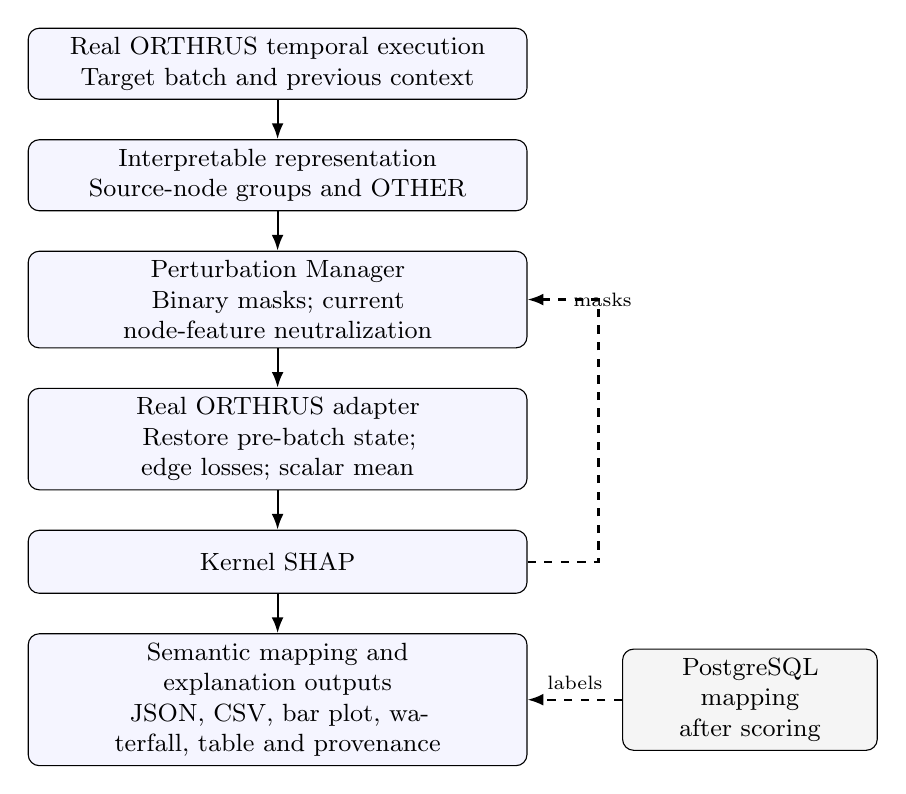
\begin{tikzpicture}[
  box/.style={draw,rounded corners,align=center,text width=6.1cm,
              minimum height=8mm,font=\small,fill=blue!4},
  flow/.style={-{Latex[length=2mm]},thick},
  node distance=5mm]
\node[box] (runtime) {\ArchRuntime};
\node[box,below=of runtime] (builder) {\ArchBuilder};
\node[box,below=of builder] (mask) {\ArchMask};
\node[box,below=of mask] (adapter) {\ArchAdapter};
\node[box,below=of adapter] (shap) {Kernel SHAP};
\node[box,below=of shap] (output) {\ArchOutput};
\node[draw,rounded corners,align=center,text width=3.0cm,font=\small,
      right=12mm of output,fill=gray!8] (db) {\ArchDB};
\draw[flow] (runtime)--(builder);
\draw[flow] (builder)--(mask);
\draw[flow] (mask)--(adapter);
\draw[flow] (adapter)--(shap);
\draw[flow] (shap)--(output);
\draw[flow,dashed] (db)--node[above,font=\scriptsize]{\ArchLabels}(output);
\draw[flow,dashed] (shap.east)--++(9mm,0)|-
  node[pos=.75,right,font=\scriptsize]{\ArchCoalitions}(mask.east);
\end{tikzpicture}
}
\caption{Final pipeline. Every mask is evaluated through the same adapter and
pre-batch state. PostgreSQL mapping supplies labels after the numerical SHAP
calculation; it does not feed a different score into the model.}
\label{fig:architecture}
\end{figure}

The responsibilities are deliberately separate. The adapter layer handles
model access and score reduction. The perturbation layer handles grouping and
current input changes. Preprocessing provides the case and mapping contracts,
while the XAI layer manages explanation and output. This separation makes it
possible to inspect a score problem without changing the plotting code, or a
mapping problem without changing inference. The dummy path remains a small
regression facility, not an alternative source of real experimental results.

\subsection{Why a custom ORTHRUS adapter was needed}
Kernel SHAP needs a function that returns one number for each mask. ORTHRUS does
not naturally expose that simple interface for this task. Its conceptual real
call is \code{model(batch, full_data, inference=True)}. The current batch and
historical data both matter, and the output is a vector of edge losses rather
than one final explanation score. Passing that vector directly to SHAP would
change the question into a multi-output explanation.

The adapter makes the selected question explicit. It calls real inference,
checks that the returned values form a valid per-edge loss vector, checks their
number against the batch, and computes their mean. The initial real integration
confirmed that a batch of 1,024 edges returned 1,024 loss values. This established
the edge/loss correspondence needed before reducing them to a scalar.

Keeping all edge positions is also important for the reduction. A neutralized
component does not remove its loss terms from the mean. Every mask still asks
for 1,024 losses and uses the same denominator for these selected batches.
Otherwise a lower score might partly come from averaging a smaller selection
rather than changing current information. The adapter and perturbation rules
work together: one preserves a fixed numerical interface, the other preserves
the structural input on which that interface is evaluated.

The mean treats every edge position equally in this batch-level question. A
component with many edges can influence several terms in the average, while a
component with few edges can still matter if its current features strongly
change the model response. A SHAP contribution is therefore not a per-edge
loss copied into a new table. It is a contribution to the response of the
whole batch under the defined feature interventions.

I kept this scalar distinct from the full official detector decision. Official
node scoring and thresholds answer a different question. The adapter does not
add a detection threshold, convert the mean into a probability or turn it into
a node label. This avoids attaching a security meaning that is not present in
the interface. The model remains unchanged; the adapter defines the numerical
quantity that the explanation is intended to describe.

\subsection{The temporal-state problem}
ORTHRUS is temporal. An inference call is not simply a calculation on an
independent row of data: it also advances temporal state. The setting
\code{inference=True} does not mean that the model becomes stateless. This is
one of the most important differences from a simple tabular SHAP example.

Consider evaluating mask A and then mask B. Without state restoration, A can
change the temporal memory before B is called. B would then be evaluated after
an extra execution of the target batch. A different score could reflect a
different history rather than the feature difference between A and B. Changing
the order of mask evaluation could also change which history each mask sees.
That would make the explanation depend on the explanation procedure itself.

The final solution is to prepare the correct real history and capture it
immediately before the target batch. Before every mask evaluation, the adapter
restores that snapshot. It runs the modified batch once and restores the same
snapshot again afterwards. The next coalition therefore begins from the same
point. The principle is simple: different current mask input, same temporal
history.

The implementation captures the relevant LastNeighborLoader state and the
GraphReindexer feature caches. These are model-specific parts of the integration,
not extra SHAP features. Their role is to keep the comparison controlled.
There is one prepared model and one reference state for the explanation, rather
than a new and possibly different runtime for every mask.

Simply calling a reset operation would not solve this problem. Resetting would
erase the actual events that preceded the target. The result would describe a
batch with empty history, not the selected batch in the reproduced experiment.
Restoration preserves the correct previous history while undoing only the
state changes introduced by the mask evaluation. This is why preparation and
restoration are separate steps, and why both are needed.

\subsection{Official temporal preparation of the target}
The target batch cannot be selected in isolation just because its file and
coordinates are known. Its score depends on what ORTHRUS has already processed.
A successful forward call on a directly selected batch is useful as a basic
integration check, but does not by itself establish the right temporal context.
The final explanation path therefore includes official temporal preparation.

Preparation starts from the training checkpoint's temporal state. The framework
checks that this memory agrees with the loaded training history. It then
processes the validation and test prefix in the original order until the target
is reached. For the first test batch, this includes the required validation
prefix. For a later test batch, it also includes earlier test batches.

The target itself is not evaluated before the SHAP snapshot is taken. This
boundary matters: the snapshot must represent the state before observing the
target, not a state that already contains it. Otherwise even the all-observed
mask would answer a different temporal question. Target selection therefore
means stopping at the right point in the sequence, not merely extracting the
right number of edges.

This preparation is performed once for an explanation. The prepared state is
then reused through snapshot restoration. Replaying the entire prefix for each
coalition would repeat substantial work without changing the intended history.
A saved coordinate still needs its checkpoint, artifacts and configuration to
identify the actual case. Graph and batch numbers alone are not a complete
description of a temporal model input.

Loading the complete THEIA\_E5 training, validation and test temporal data
caused excessive host RAM use. Upstream ORTHRUS also materialized
\code{full_data.msg}. The real experimental configuration uses
\code{edge_features=edge_type}, so the local data-loading patch avoids
materializing \code{full_data.msg} when messages are not required. Historical
timestamps and edge types remain concatenated in their original order.
This was a runtime and memory compatibility change, not a change to the GNN
architecture or the intended numerical features used in the tested path.

\subsection{Choosing interpretable components}
Each selected batch contains 1,024 edges. Making every edge an independent
component would create a very large binary space and a long explanation.
An analyst would also have to connect many separate edge values back to the
same recurring entities. The project therefore needed a smaller representation
that remained connected to the current batch.

The builder supports several possible grouping strategies, including individual
edges, source nodes, edge types and time chunks. The real final experiments use
source-node grouping. Every component collects the batch edges with one source
ID. This makes the group easy to relate to an entity while retaining a clear
mapping back to the assigned events. The source can be a file, a subject or a
netflow; it is not necessarily a process.

The final limit is eight components. If there are more source groups, the
largest are kept separately and the remaining smaller groups are combined into
OTHER. This choice is based on the number of assigned edges, not on exported
malicious labels, score or expected SHAP value. The explanation does not use
known labels to choose which entities receive separate contributions.

Eight components give $2^8=256$ possible masks. This small finite space made
complete coalition evaluation practical for the selected final runs. It also
keeps the figures readable. The component order is fixed throughout scoring,
so that a mask position always means the same component. Sorting the final
ranking changes presentation, not the meaning of earlier masks.

The trade-off is reduced detail. OTHER is one component and gets one value even
when it contains many sources. It avoids discarding the remaining edges, but
cannot show which member of the aggregate is responsible for its contribution.
The case analysis must therefore consider both the SHAP value and the size of
the group. Small contributions do not automatically mean small groups, and a
large aggregate is not a single entity.

\subsection{Why edge deletion was rejected for real explanations}
Removing an edge or a whole source group is an intuitive starting idea. The
result looks like a smaller graph, and an absent event seems easy to explain.
For the real ORTHRUS path, however, removal changes more than the current
information whose effect is being studied.

Deleting edges changes graph structure, the local sequence and positions, and
the relation between the current input and temporal history. ORTHRUS uses
ordered events and temporal neighborhood information. A local slice can look
structurally valid while no longer matching the history assumed by the runtime.
A score difference would then mix a feature intervention with a different graph
and a different temporal alignment.

The normal explanation therefore does not delete edges. The target keeps the
same source/destination structure and the same number and order of events for
every mask. Its features change, but it remains the same structural and temporal
problem from the model's point of view. This gives a clearer interpretation to
the score differences.

\subsection{Why targets and historical edge types remain unchanged}
The decoder used in the reproduced instance predicts edge type. The observed
edge type is therefore a target against which a loss is calculated. Setting
\code{batch.edge_type} to zero would not be a neutral feature change. Depending
on target handling, an all-zero vector can be converted by argmax into a real
class. That would silently replace the observed event type rather than remove
its information in a controlled way.

The framework therefore keeps current edge types unchanged. Every coalition is scored
against the same observed targets. The question becomes how the current node
features affect prediction of those targets, not how the score changes when
both inputs and answers are rewritten. Keeping the target fixed also makes
the per-edge losses comparable across masks.

Historical context must stay fixed for a related reason. The historical
\code{e_id} values sampled by ORTHRUS refer to previously inserted edges.
They are not local row numbers of the current batch. Using them to modify
\code{full_data.edge_type} for a current masked component could alter unrelated
past events. That would change the history on which the target prediction is
conditioned.

The normal rule is consequently to preserve both the current targets and the
historical edge types. The explanation is about current node features given
the real previous history. It is not a claim about deleting the entire history
of an entity. This distinction is important when a component is neutralized
but the same entity has appeared earlier in the execution.

\subsection{Final neutralization semantics}
The final Perturbation Manager changes only current \code{x_src} and
\code{x_dst} node-feature inputs. For an inactive component, the relevant
current feature vectors are replaced with zeros. A mask value of 1 keeps the
component observed; a value of 0 applies this neutralization. Each evaluation
starts from the original batch, rather than modifying a batch left over from
an earlier mask.

The manager keeps source and destination IDs, edge count and order, timestamps,
edge types, message/target structure and full historical context unchanged.
It does not recompute the original Word2Vec embeddings for every coalition.
The intervention is on the extracted current node features consumed by the
real inference path. This is a narrower question than changing raw commands
or rebuilding provenance data.

These rules define the SHAP game used by the project. They are not only
implementation safeguards: choosing a different perturbation would change the
function being explained. For example, removing events or changing historical
features could produce different contributions even with the same SHAP backend.
The report therefore interprets values only under the final current-feature
neutralization policy.

The all-zero mask means that all interpretable current components are
neutralized while graph and history remain present. It is not an empty graph,
a benign batch or an attack-free system. The reference score may be larger than
the original score, as it is in the five selected cases. That outcome is allowed
by the definition and must not be corrected or renamed to fit a benign-baseline
interpretation.

\subsection{Handling repeated nodes consistently}
The same source or destination can appear in several rows of a batch. If only
one row were neutralized, another current occurrence of the same node in the
same role could retain or overwrite its representation inside ORTHRUS. The
mask would then have an effect that depended on which occurrence was consumed,
rather than consistently removing that node's current feature information.

The final policy neutralizes all current occurrences of the selected node in
the same role. Source and destination roles remain distinct. Neutralizing a
source does not automatically neutralize every destination occurrence of the
same ID. The policy follows the roles consumed by the model and does not
recursively spread through the graph.

A shared destination can still connect interventions from different source
groups. If two source groups point to the same destination, disabling one group
can neutralize that destination's current-role features on rows assigned to
the other. This does not mean the edge partition is broken. The partition
identifies components; the perturbation rule determines their feature effects.
The two need not be independent.

This is why the final outputs distinguish assigned edges from the feature rows
affected by an intervention. An assigned-edge count shows how the component
was built, not that every model effect is confined to those rows. SHAP compares
all combinations under the same rule, so the resulting contributions describe
this consistent repeated-node policy. They should not be read as independent
causal effects of individual events.

\subsection{Kernel SHAP integration and score reconstruction}
Kernel SHAP operates on a vector of eight binary entries. The all-zero mask
provides $f(0)$, the neutralized reference. The all-one mask provides $f(1)$,
the original score. Intermediate masks keep different subsets observed.
Every score uses the same adapter, reduction, targets and pre-batch history.
The framework caches scores within an explanation so that a mask requested
again does not require another target evaluation.

Kernel SHAP assigns a signed contribution $\phi_i$ to component $i$. The
reconstructed score is the reference plus all contributions:
\[
  f(1)\approx f(0)+\sum_i\phi_i.
\]
The original score is measured by ORTHRUS with all current components observed.
The reconstructed score is computed from the reference and component values.
Comparing them is a direct check that the explanation accounts for the selected
scalar response.

All final runs have eight components and 256 unique evaluated masks. Kernel
SHAP was run over the complete coalition space. The saved diagnostics also
separate the internal coalitions from the two endpoints. There is no need to
interpret the requested sample count as an estimate of total runtime: preparing
the earlier temporal sequence is separate work.

A positive contribution raises the score relative to $f(0)$; a negative
contribution lowers it. Neither sign classifies an entity. In particular,
negative does not mean benign. Different cases have different references, so
the sign or magnitude cannot be read without that case's $f(0)$. The residual
checks local score reconstruction, not published detector accuracy. Complete
mask coverage does not change the meaning or limits of the chosen reference.

\subsection{Semantic mapping after scoring}
A raw explanation can identify a component as \code{node:1301224}, but that ID
alone gives little help to a reader. After SHAP calculation, PostgreSQL mapping
adds entity and event metadata. It can identify the entity type, file path,
process command, event operation and relations to other entities. For example,
node 1301224 becomes a file associated with \path{/etc/hosts}.

This step is performed after the numerical explanation. It does not alter the
mask scores or recalculate the SHAP values. The model does not use the new
readable labels as additional inputs during explanation. Keeping mapping out
of the scoring loop also avoids repeating metadata queries for every mask.
The same score can therefore be inspected before and after enrichment.

Mapping preserves distinctions that matter in the results. A subject and a file
can have the same path but remain different nodes with different roles. Several
Firefox subjects can share an executable label while receiving separate
component values. Event operations explain the recorded interactions without
turning each event into an independently attributed component.

The final JSONs preserve mapping quality and provenance as well as labels.
Ambiguous or missing identities must remain visible instead of being replaced
with a convenient guessed name. An offline metadata backend is also supported,
but the saved five final cases report PostgreSQL enrichment. This semantic
layer makes the results useful for inspection; it does not certify that a
familiar process name is safe or that an unfamiliar name is malicious.

\subsection{Explanation records and four visual outputs}
The complete machine-readable record is \code{result.json}. It preserves the
reference and original scores, component order, signed contributions, ranking,
reconstruction diagnostics and mapping metadata. It is the source for exact
values when a plot rounds labels. CSV exports provide a convenient numerical
view for comparison and reporting without needing to read a large JSON.

The SHAP bar plot ranks components by absolute contribution while keeping their
signs. It quickly identifies dominant components and opposing effects. Ranking
by absolute value does not mean all large values raise the score: a large blue
negative bar can be the main feature of a high-score case. The bar plot is
useful for inspecting the pattern, not for making a separate detector decision.

The waterfall starts from $f(0)$ and adds the component values in presentation
order. It ends at the reconstructed score and shows original $f(1)$ separately.
This makes the reference, total change and local reconstruction visible in one
view. The displayed path is an accounting of contributions, not the time order
of events or a sequence of intermediate attacks.

The summary table combines component identity, semantic label, assigned-edge
count and signed SHAP value. The saved CSV retains detailed values, operations
and counterparts, while PNG/PDF versions provide a shareable visual table.
This view is useful when exact group sizes matter or several components have
similar names. It complements the ranking rather than replacing it.

The SHAP-attributed provenance subgraph connects important component nodes to
counterpart entities and event types. Only component nodes carry SHAP values.
Counterparts and edges provide context: they help show which recorded
interactions belong to the component. They do not receive new independent
attributions. The graph presents a limited readable view, while the table and
JSON retain the complete component list. The experimental section uses saved
examples of all four views to show when each is informative.

\section{Experimental Results and Analysis}
\subsection{Full THEIA\_E5 test scan}
Running a full explanation for every test batch would repeat many target
inferences and produce more detailed results than were needed for the project.
The scan was introduced to separate broad score inspection from detailed local
explanation. It runs ORTHRUS over the complete test split without SHAP masks,
records the batch means and descriptive endpoint membership, and provides a
basis for selecting interesting cases.

The scan follows the temporal sequence. Starting from verified checkpoint
history, it processes the validation prefix and then the test batches in order.
Unlike SHAP evaluation of a single target, it does not restore the pre-batch
snapshot between successive scan batches. Each batch must advance the state
for the next one. The scan and explanation modes therefore share runtime
preparation but use state differently for different purposes.

The scanner saves one row per test batch, including its coordinates, edge
count and loss statistics. This makes a suggested case traceable to the same
position later used by the explanation configuration. The distribution is a
distribution of batch means, not one pooled loss over every test edge. The
recorded edge counts allow the total coverage to be checked separately. The
five explained batches each have 1,024 edges; the scan totals describe the
complete split, including its batch boundaries.

The saved scan is complete and contains \ScanBatches{} test batches and
\ScanEdges{} edges. Their score distribution is shown in Table~\ref{tab:scan}.
The overall mean, about 0.347405, is below the median, about 0.412648. The lower
quartile is close to the minimum, while upper percentiles show a higher-score
part of the test set. This made it useful to select cases from several regions
rather than treating one integration example as representative of every batch.

\begin{table}[htbp]
\centering
\begin{tabular}{lr}
\toprule
Statistic of test-batch mean losses & Saved value\\
\midrule
Minimum & 0.0033847622\\
Maximum & 1.7857131806\\
Mean & 0.3474048767\\
Median & 0.4126481353\\
25th percentile & 0.0037371573\\
75th percentile & 0.6949211438\\
90th percentile & 0.6966610471\\
95th percentile & 0.6999841991\\
99th percentile & 0.9773277887\\
\bottomrule
\end{tabular}
\caption{Distribution from the completed saved THEIA\_E5 test scan. These are
statistics of batch-mean losses, not official node-level detector metrics.}
\label{tab:scan}
\end{table}

The exported malicious-node set contains 70 IDs. There are 246 scan batches with
at least one endpoint in that set. Within this group, the mean is about 0.719045,
the median about 0.696006, the minimum about 0.047847 and the maximum about
1.785713. Without membership, the mean is about 0.340920, the median about
0.370385 and the maximum about 1.782047. The groups differ, but their score
ranges overlap substantially.

This is descriptive membership, not a classification rule. A node can occur in
many events and batches, and its presence does not label every event in the
batch as an attack. High score and membership are not equivalent: a high score
occurs without membership, and a very low score occurs with it. The scan does
not compute official detector performance. It characterizes the reproduced
instance's batch scores and helps decide which ones to explain.

\subsection{Case-selection strategy}
Five cases were retained for detailed analysis. Their coordinates are stored in
the final experiment configurations, so that the selected batch is explicit.
The selection compares three things: score magnitude, exported-node membership
and attribution structure. It is a deliberate set of examples, not a random
sample for estimating overall explanation quality.

Initial validation uses test graph 0, batch 0. It is the first complete real
explanation used to check the final integrated path. It brings together official
history preparation, the 1,024-edge/1,024-loss correspondence, component masks,
state restoration, mapping and output. Its role is a clear reference case, not
the claim that it has the most interesting security score.

The high malicious-related case is test graph 40, batch 0. Its scan score is the
highest overall and it contains one source node in the exported set. Test graph
35, batch 82 is the high-score case without membership. The two explanation
scores are both around 1.78, making them useful for asking whether similar
numbers also have similar local explanations.

The low malicious-related case is test graph 98, batch 39. It contains membership
but has a score around 0.047847, at the low end of that descriptive group. The
median reference is test graph 42, batch 35, with score around 0.412555. It was
selected as the available batch closest to the global scan median. It is not
claimed to be exactly equal to that median.

The scan does not launch SHAP automatically. A suggested extreme or median
coordinate becomes an explanation only after it is selected and configured.
This keeps the broad scan separate from the expensive local study. The initial
validation case adds a known integration reference to the distribution-based
choices; it was not selected because it was an extreme. Keeping both purposes
in the final set makes the comparison easier to explain.

All five final explanations use eight components, 1,024 edges and 256 unique
masks. This common setup makes their local patterns easier to compare. It does
not mean their feature reference states have the same score. Each batch has its
own $f(0)$, so absolute score, reference and contributions must be read together.

\subsection{Local reconstruction across the five cases}
Table~\ref{tab:cases} summarizes the reference, original score and contribution
sum. The scores here come from the explanation JSONs. The separate scan provides
the membership information and selection context. Its scores agree closely
with the explanation runs, but they are saved results from different executions
and need not be numerically identical.

\begin{table}[htbp]
\centering\small
\setlength{\tabcolsep}{4pt}
\begin{tabular}{@{}lccrrr@{}}
\toprule
Case & Test G/B & Member & $f(0)$ & $f(1)$ & $\sum\phi_i$\\
\midrule
\CaseRowsEN
\bottomrule
\end{tabular}
\caption{Five final saved explanations. G/B indicates test graph/batch. Member
means that an endpoint is in the exported node set, not a label for the batch.
Values are rounded to six decimals.}
\label{tab:cases}
\end{table}

The saved reconstruction residual is zero in four cases and approximately
$\MaxResidual$ in initial validation. Thus $f(0)+\sum_i\phi_i$ reconstructs
the original model score with zero or negligible residual. This is useful
evidence of local explanation fidelity with respect to the model instance
actually executed. The values have not been adjusted to make a plot end at
the desired score.

All five sums are negative. In each case, the original current features lead
to a lower score than the fully neutralized reference. This common direction
is an observation about these five selected games, not a general rule about
ORTHRUS or the full test set. It does not mean that any selected activity is
benign.

Complete mask coverage makes the case comparison stronger than a comparison
based on a small unvisited part of the coalition space. It still answers the
chosen feature-intervention question. Local reconstruction does not validate
detector accuracy, the exported labels or the suitability of the reproduced
features for the pretrained model. Those are different questions and remain
separate in the limitations.

\subsection{Initial validation: a complete readable example}
The initial case has $f(0)=\InitialReference$, $f(1)=\InitialOriginal$ and total
contribution \InitialSum{}. Every individual contribution is negative. The
observed current features therefore reduce this batch score compared with the
reference in which all current components are neutralized. The reduction is not interpreted
as benign activity.

The ranking starts with OTHER, which contains 14 source nodes, 383 assigned
edges and a contribution about $-0.059756$. The next component is file node
1301260, mapped to \path{/proc/stat}, with 186 edges and contribution about
$-0.017277$. These two groups account for much of the total reduction, but they
are different kinds of explanation unit: one is an aggregate and one a single
source entity.

The remaining separate source groups are \path{/proc/1486/net/sockstat}
($-0.011965$), \path{/proc/1486/net/arp} ($-0.010802$), \path{/proc/loadavg}
($-0.004075$), \path{/proc/1486/net/dev} ($-0.003639$), \path{/proc/meminfo}
($-0.002780$), and \path{/proc/1350/stat} ($-0.002124$). Their common negative
direction is easy to miss if one reads only the original scalar. The mapping
also makes clear that these components are files, not eight independent
processes.

Table~\ref{tab:initial} keeps the values and group sizes together. It is useful
for a direct numerical check and includes every component. The actual saved
visual summary in Figure~\ref{fig:summary} adds operations, counterpart entities
and mapping status. The CSV remains the source for full precision and labels;
the figure is a readable sharing/reporting view of the same explanation.

\begin{table}[htbp]
\centering\small
\setlength{\tabcolsep}{5pt}
\begin{tabular}{@{}llrr@{}}
\toprule
Semantic name & Source ID & Edges & SHAP\\
\midrule
\InitialSemanticRowsEN
\bottomrule
\end{tabular}
\caption{Initial-validation components, derived from the saved summary CSV.
Edge counts describe assigned current events, not separate event attributions.}
\label{tab:initial}
\end{table}

The assigned-edge counts also help interpret the ranking. OTHER and the
proc-stat group cover 569 of the 1,024 assigned positions together. That is
substantial coverage, but the edge count alone does not compute their SHAP
values. Their current features interact with the model and the other masked
groups. A reader should therefore use the table to understand the grouping,
not treat the counts as a second estimate of feature importance.

This case demonstrates why mapping is part of the final workflow. The node ID
1301260 alone says little, while the path and recorded operations explain which
input group was affected. Its provenance links include
\path{/usr/bin/prometheus-node-exporter} subjects. That name helps describe the
recorded interaction; it does not establish a security verdict. The same rule
applies to the other familiar-looking paths.

\newgeometry{margin=10mm,footskip=5mm}
\begin{landscape}
\begin{figure}[p]
\centering
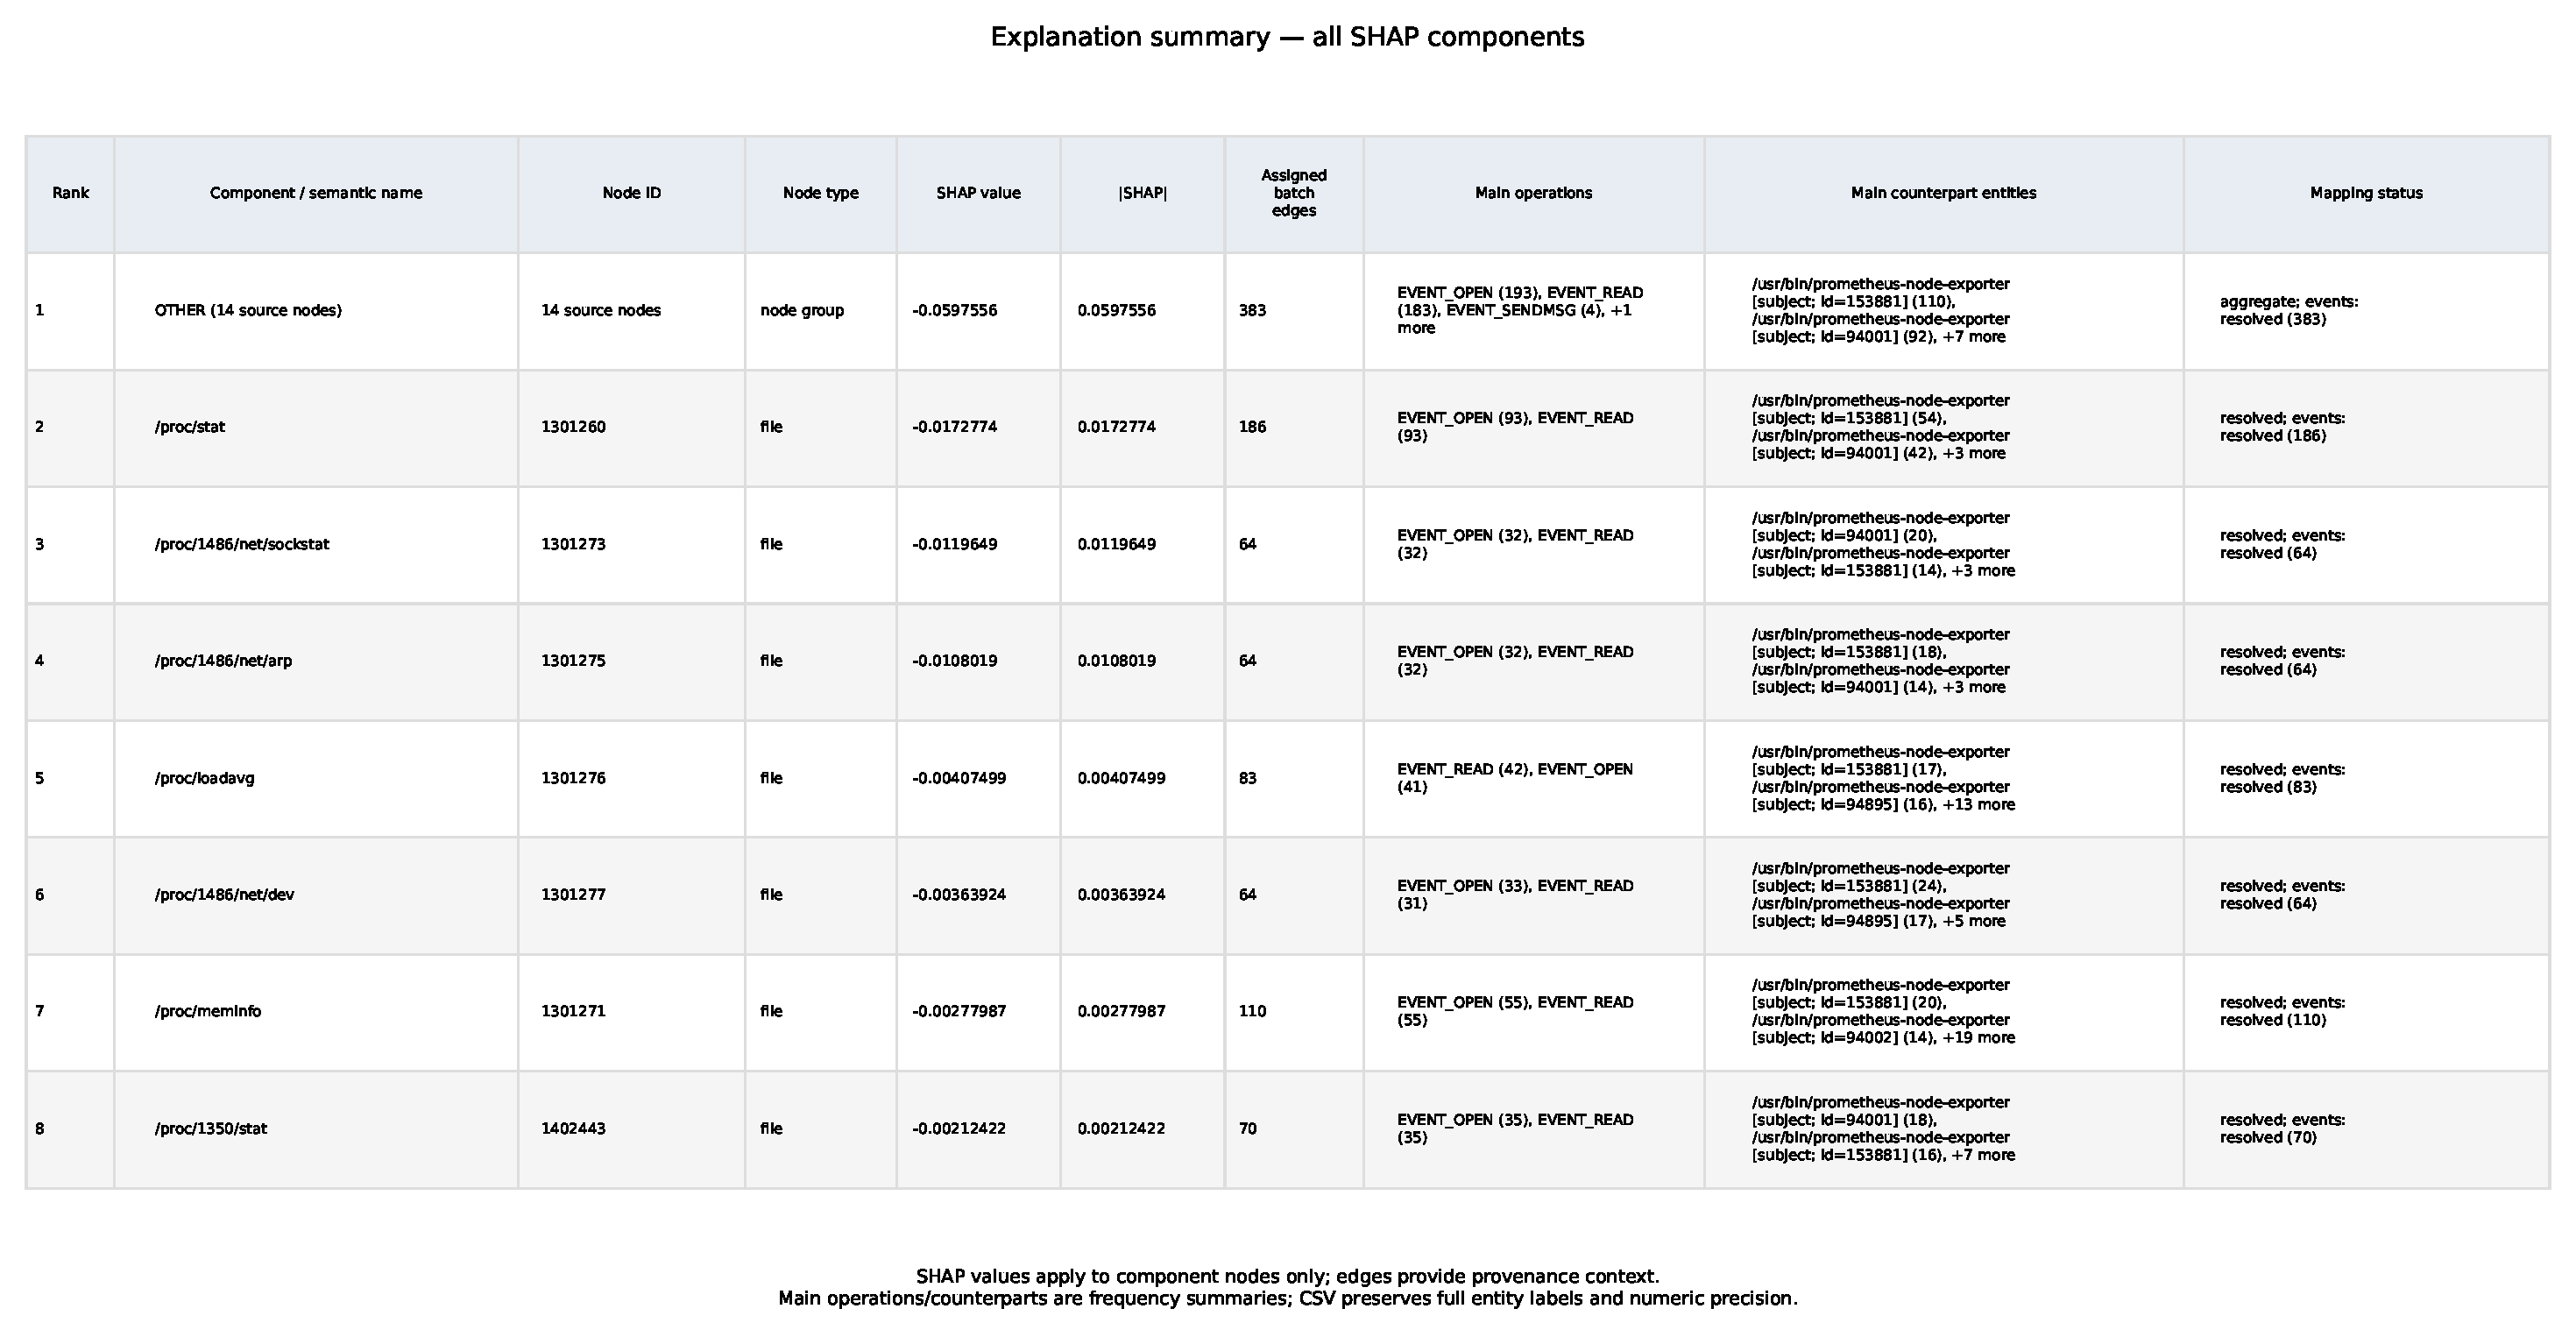
\includegraphics[width=\linewidth,height=.88\textheight,keepaspectratio]{figures/initial_summary_table.pdf}
\caption{Actual saved initial-validation summary-table visualization, shown
complete in landscape format. It combines labels, source identities, signed
values, edge counts, operations and counterparts. It is an explanation table,
not a list of detected attacks.}
\label{fig:summary}
\end{figure}
\end{landscape}
\restoregeometry

\subsection{High malicious-related score: opposing contributions}
The high malicious-related case has $f(0)=\HighMemberReference$ and
$f(1)=\HighMemberOriginal$. Its total contribution is \HighMemberSum{}.
Although its original score is high relative to the scan, the total effect of
its observed current features is negative relative to its own higher reference.
A high score therefore does not require all component values to be positive.

The main contribution is the file \path{/etc/hosts}, about $-0.302713$. The
subject \path{/usr/bin/whoopsie} contributes about $+0.101541$. The latter partly
offsets the former. These two values show a clear opposition within the same
batch. Describing the case only as ``high anomaly'' loses this internal structure.

Other notable values are \path{/proc/17224/net/if_inet6}, about $-0.033405$,
OTHER, about $-0.021326$, and netflow node 40, about $-0.017363$. The netflow
remains identified as a node/type rather than being given an unverified endpoint
interpretation. The smaller file groups also contribute to the total, so the
largest bar is not the full explanation of the difference from $f(0)$.

The scan records one malicious source-node membership for this batch. In the
saved component mapping, labelled source 93983 is inside OTHER. Its individual
contribution is therefore not available. It would be incorrect to assign
OTHER's value to that node, or to identify the positive whoopsie value with the
known malicious label. Membership and the contribution ranking are different
pieces of information.

The upper bar plot in Figure~\ref{fig:highcomparison} is useful here because it
shows both signs at once. The positive contribution raises the score relative
to the reference when averaged through the SHAP game, while the strong negative
file contribution lowers it. Neither sign says whether the program or file is
benign. The plot explains the reproduced model's local response, not the cause
of the underlying activity.

\subsection{High score without membership: a different local pattern}
The second high-score case has $f(0)=\HighNoMemberReference$ and
$f(1)=\HighNoMemberOriginal$. Its final value is very close to the previous
case, but its total contribution is only \HighNoMemberSum{}. The reference is
also different. Comparing only the two final numbers would hide both facts.

OTHER is the main negative component, about $-0.169173$. The seven separate
Firefox source groups are all positive: about $+0.027870$, $+0.026751$,
$+0.021307$, $+0.016031$, $+0.009404$, $+0.008490$ and $+0.008462$. Together they
partly offset OTHER. This is a different pattern from a dominant negative
\path{/etc/hosts} contribution opposed mainly by one whoopsie component.

The positive Firefox values sum to about $+0.118315$. Combining them with
OTHER's roughly $-0.169173$ produces the small negative total, about $-0.050858$.
The final score is high even though the net change is modest, because the
reference was already high. This is different from the larger net reduction
in the membership case. The bar plot is useful precisely because cancellation
between components is not apparent from the net change alone.

Several source IDs share the Firefox executable label. Mapping should not merge
them just because their paths match. They are distinct components with different
assigned events and SHAP values. This makes the combination of node identity,
semantic label and edge count more informative than a plot that displays only
one generic application name.

\begin{figure}[htbp]
\centering
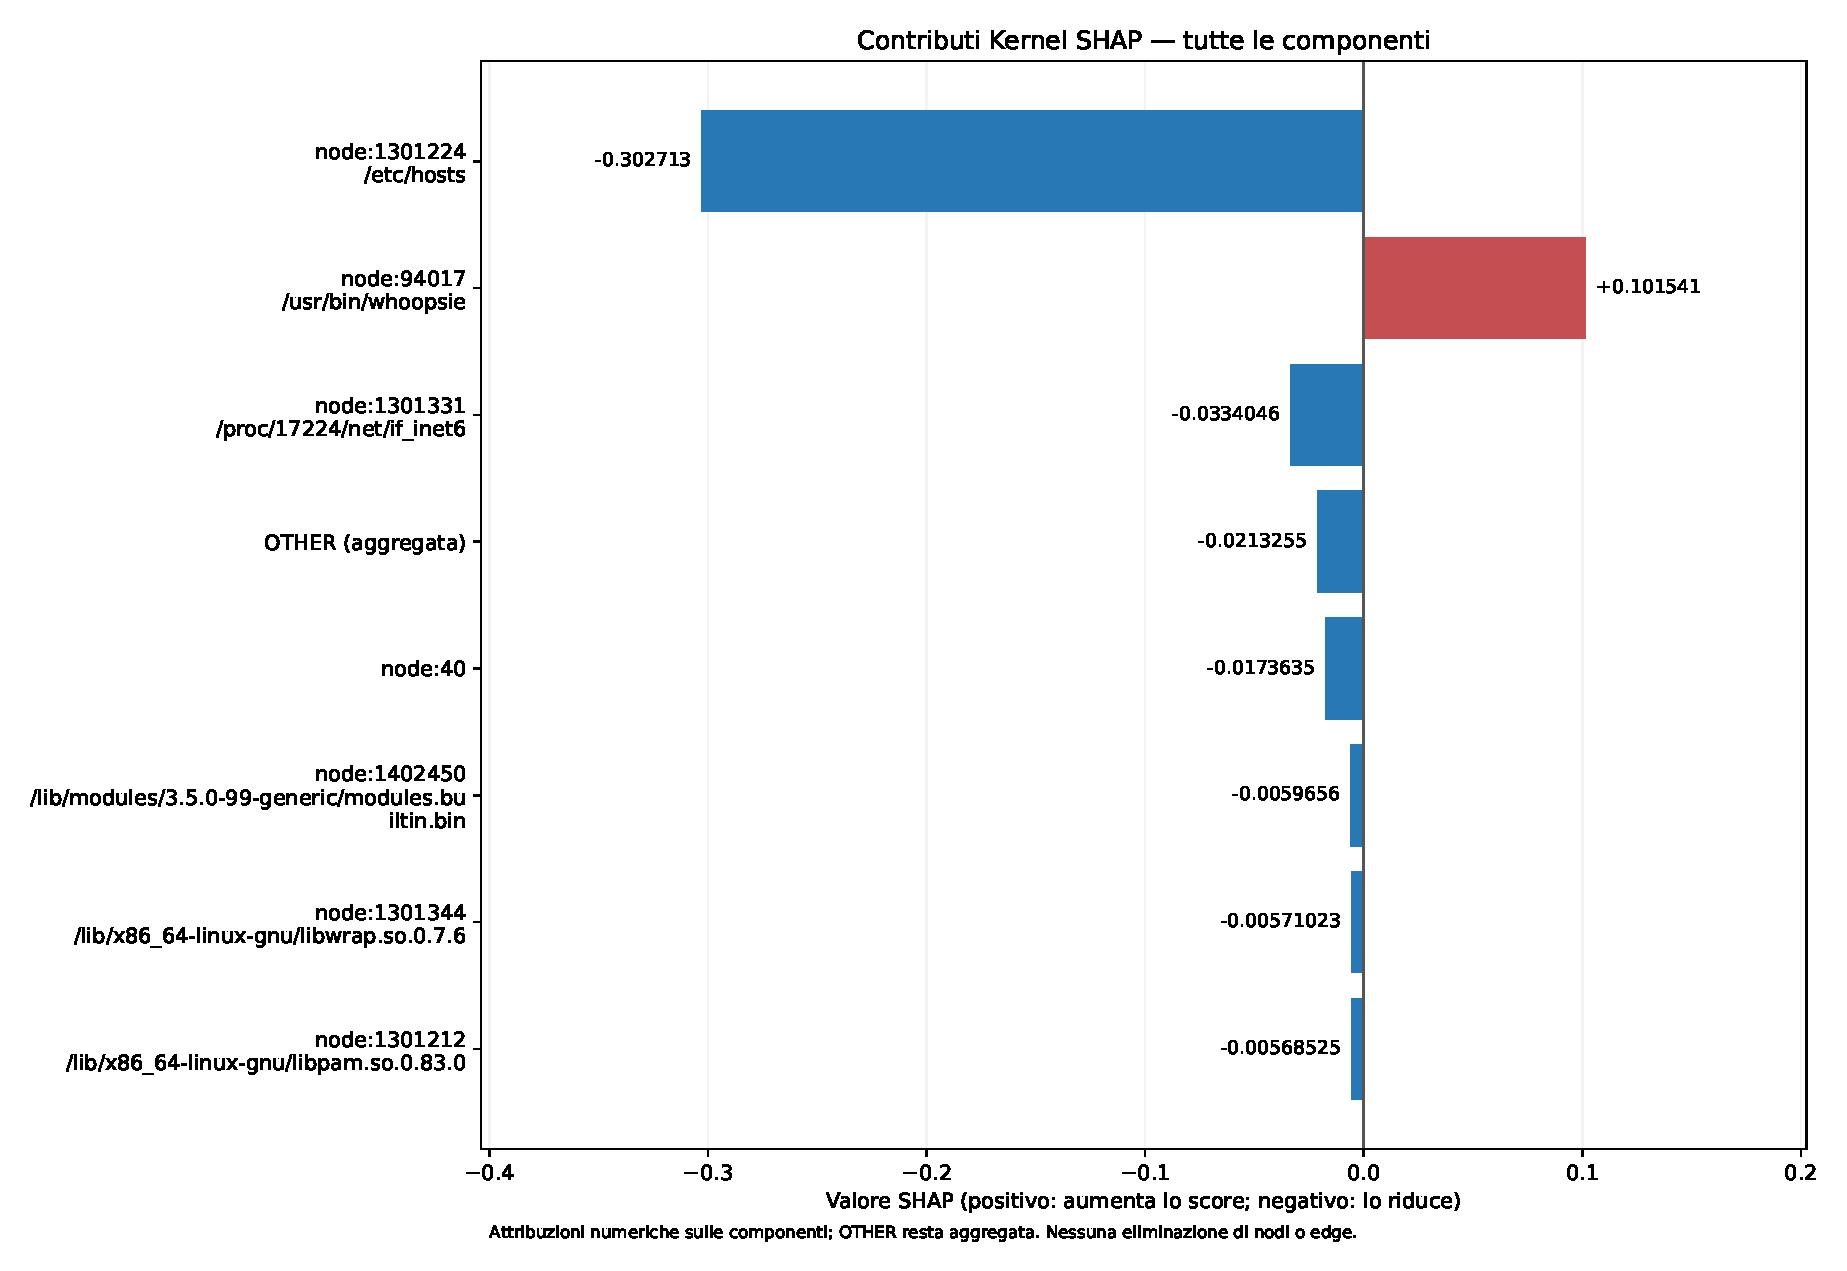
\includegraphics[width=.94\linewidth]{figures/high_malicious_bar.pdf}\par
\vspace{2mm}
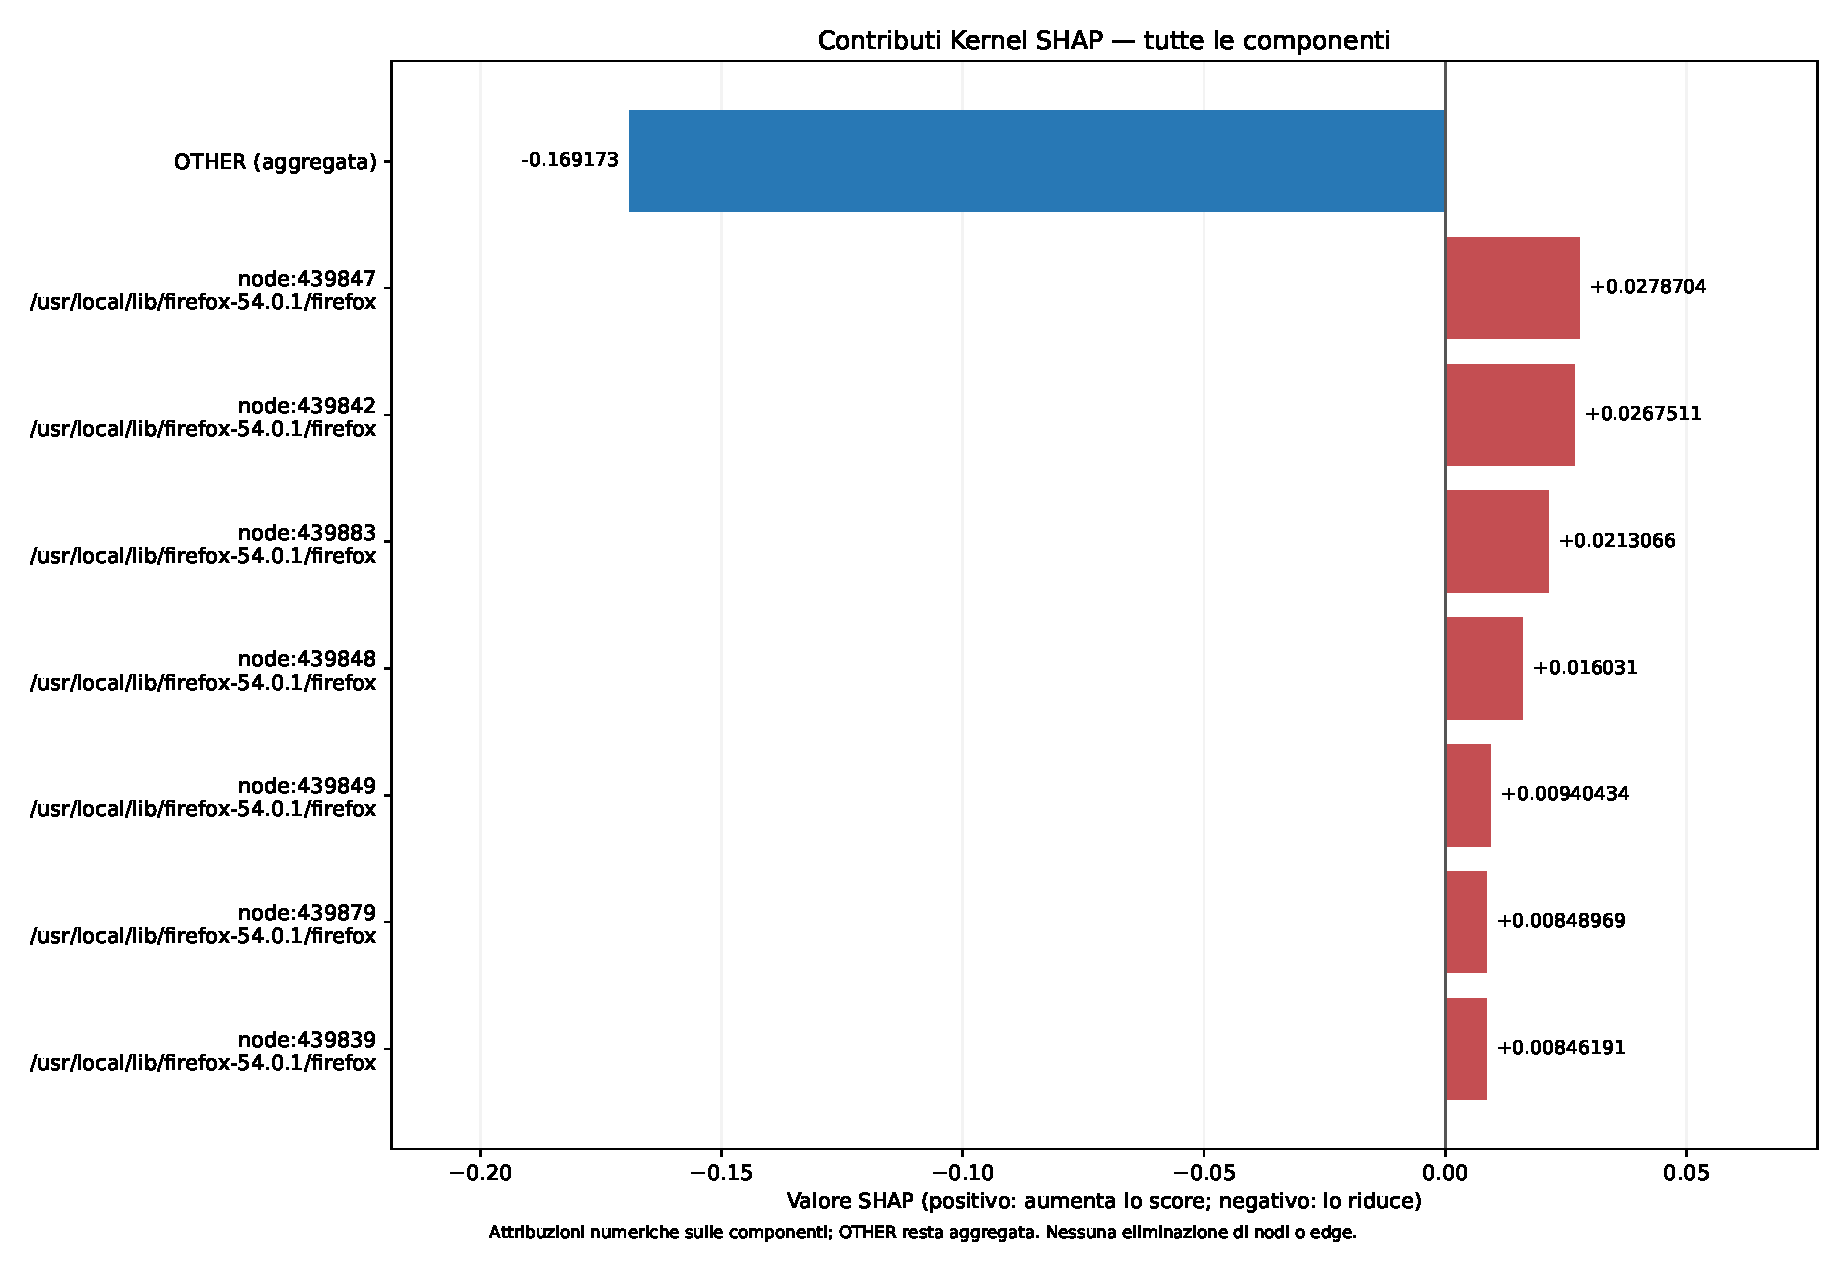
\includegraphics[width=.94\linewidth]{figures/high_no_malicious_bar.pdf}
\caption{Actual saved bar plots of the two high-score cases: membership at the
top, no membership at the bottom. Compare the opposing file/subject pattern
with the negative OTHER and positive Firefox groups. The final scores are
similar, but the local explanations are not.}
\label{fig:highcomparison}
\end{figure}

The paired plots support one of the main observations of the project: similar
anomaly scores can have very different local explanations. Their use is not to
choose a malicious program from the longest positive bar. Instead, they reveal
which current component groups move each batch away from its own reference.
The same score magnitude can be reached from different references and different
balances of positive and negative effects.

The lack of membership in this case does not certify all activity as benign.
It only states that the batch endpoints are not in the exported set. Equally,
the high score is not enough to assign an official detector outcome. The value
of this comparison is that the explanation adds structure that neither the
membership flag nor the scalar provides on its own.

\subsection{Low malicious-related score: membership with a small mean}
The low case has $f(0)=\LowMemberReference$, $f(1)=\LowMemberOriginal$ and total
contribution \LowMemberSum{}. Its scan counterpart is the minimum within the
membership group. This was selected deliberately to inspect a batch where the
presence of an exported malicious node coexists with a low mean score.

OTHER contributes about $-0.004734$. Subject node 93983, mapped to
\path{/usr/sbin/sshd}, contributes about $-0.003659$. The file with the same path,
node 1301343, contributes about $-0.002750$. The distinct types matter: a subject
and a file can share a displayed path without being the same component or the
same model input.

The following values include libwrap at about $-0.002322$, xscreensaver at
$-0.001388$, another SSH subject, node 572644, at $-0.000995$, and libpam at
$-0.000912$. The final smaller SSH group also has a negative value. All eight
contributions reduce the score relative to the small neutralized reference.
The ranking does not reveal a large positive component hidden by the sum.

The separate appearance of node 93983 is especially useful when compared with
the high malicious-related case. Here its local contribution can be inspected;
there it is inside OTHER. The same exported identity does not imply the same
current features, context, group or score in every batch. The explanation is
local to the selected current batch and its prepared history.

OTHER in this case contains 966 source nodes and 966 assigned edges. Its small
SHAP magnitude therefore must not be confused with a small aggregate. Most
source detail is hidden inside one component. The case provides evidence that
membership does not directly determine the batch mean, not an official error
classification for the detector. No batch-level detection threshold or temporal
attack label was used to reach the selection.

\subsection{Median reference: the largest reference-to-original change}
The median-reference case has $f(0)=\MedianReference$, $f(1)=\MedianOriginal$
and total contribution \MedianSum{}. Among the five cases, it has the largest
absolute total change between reference and original score. Its final score is
near the global median, not near the maximum. This separates the size of a
local explanation from the magnitude of the final anomaly score.

OTHER contributes about $-0.334073$. Three SSH subjects have values about
$-0.115993$ for node 455696, $-0.115179$ for node 456191 and $-0.115089$ for node
455944. Two run-parts groups each contribute about $-0.039548$. The remaining
file components have smaller negative values. All eight values point down from
the neutralized reference.

\begin{figure}[htbp]
\centering
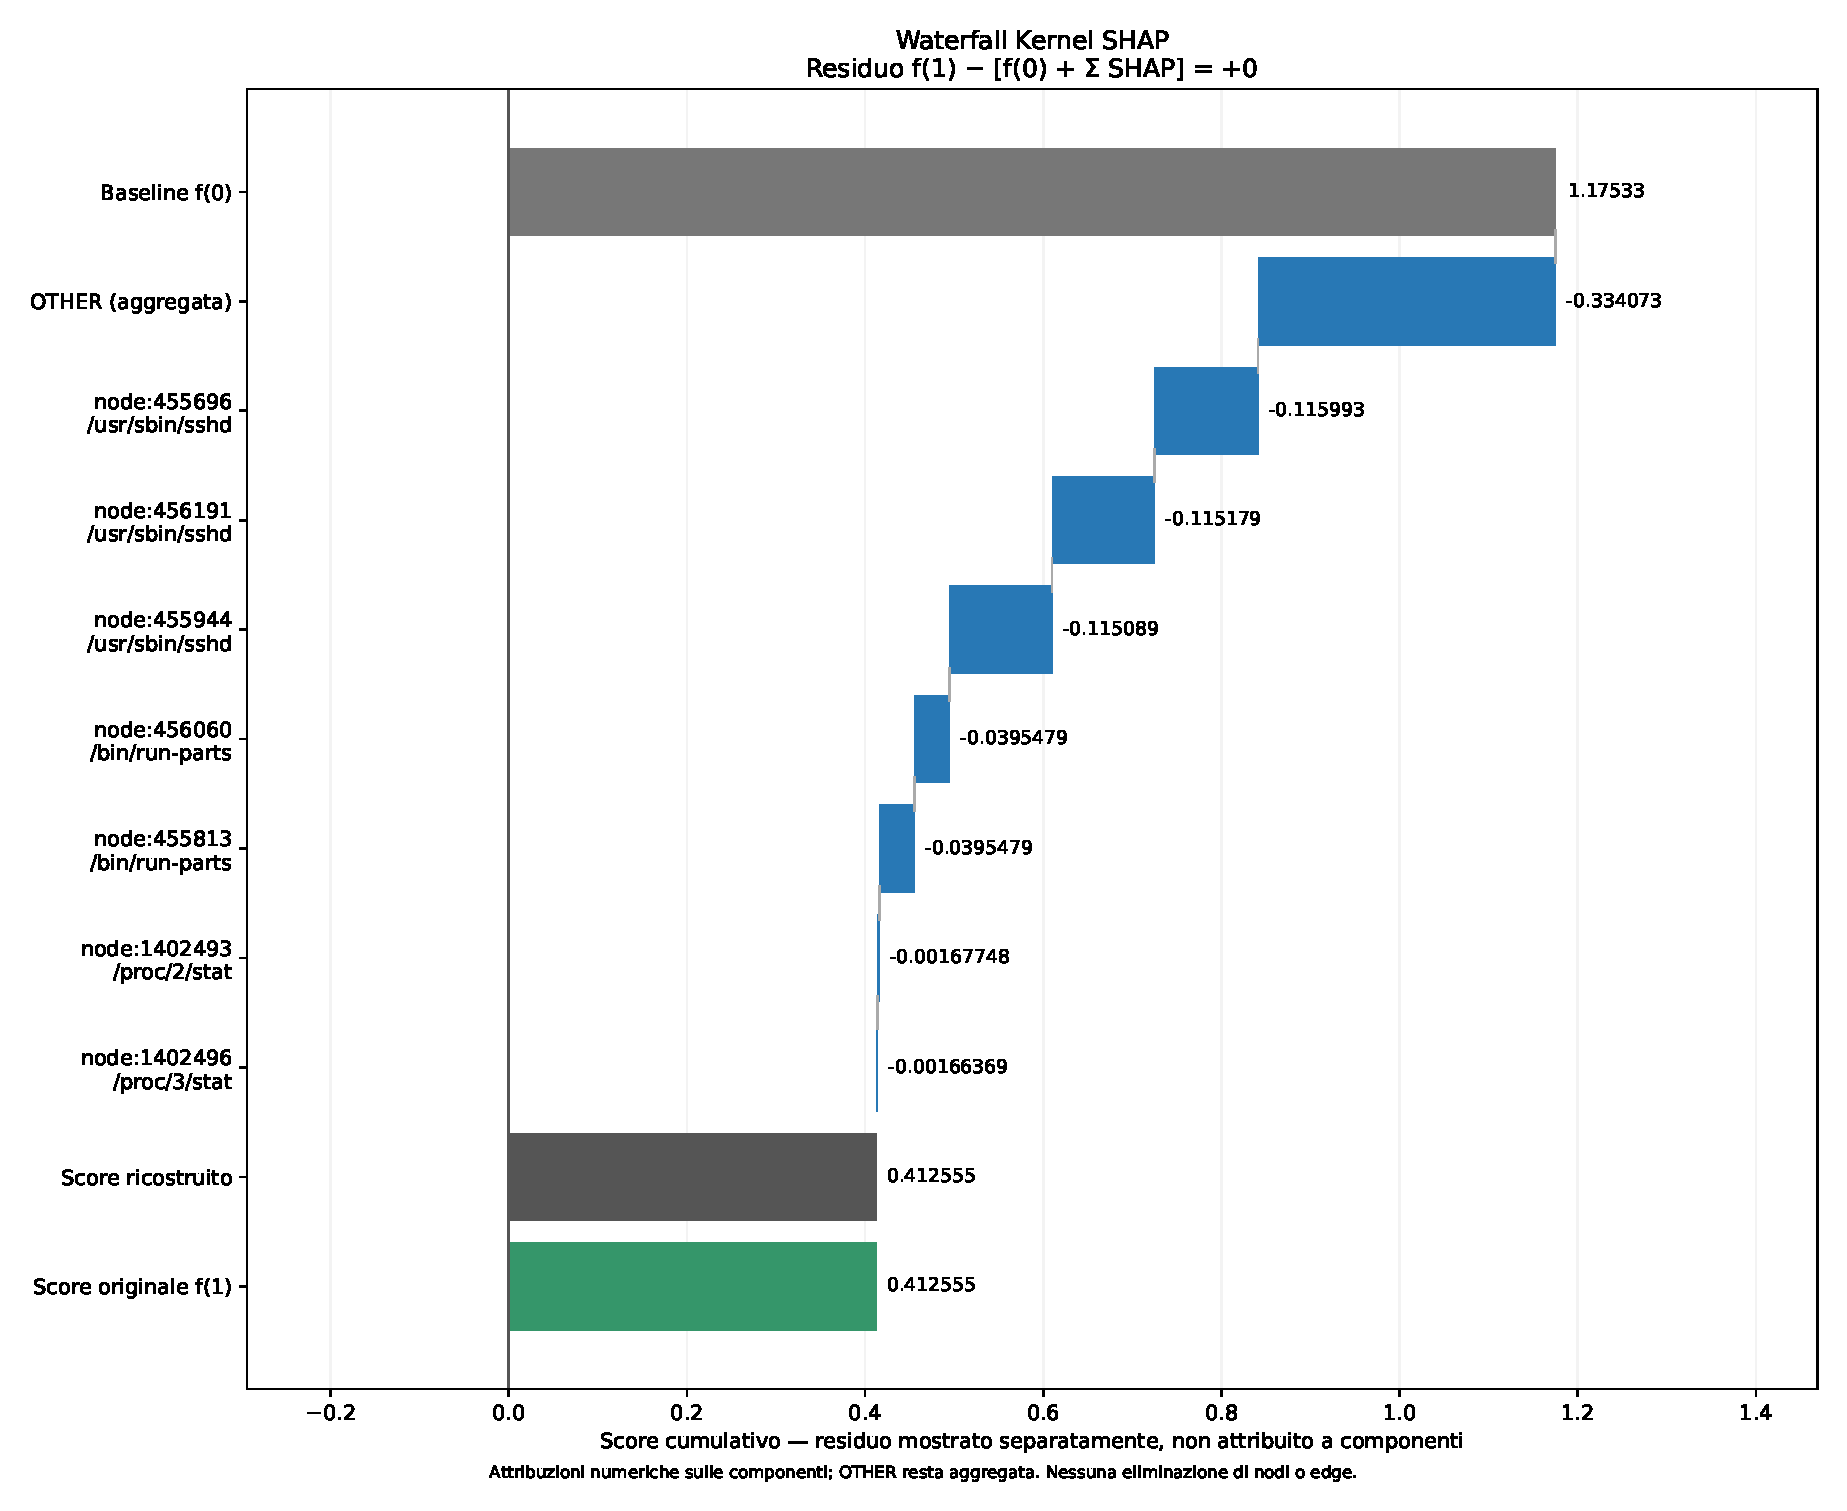
\includegraphics[width=.98\linewidth]{figures/median_waterfall.pdf}
\caption{Actual saved waterfall for the median-reference case. The plot starts
from the neutralized reference and follows every signed contribution. It shows
both the reconstructed endpoint and original model score. Their agreement is
a local additive check, not an evaluation of attack detection.}
\label{fig:waterfall}
\end{figure}

Figure~\ref{fig:waterfall} is useful because the large reduction is visible as a
sequence of component increments. Starting at about 1.175326, OTHER and the SSH
groups provide most of the movement toward about 0.412555. The reconstructed
endpoint is calculated from the contributions, while the original endpoint is
a separate model evaluation with all current components observed.

The largest individual bar and the total change also answer different
questions. OTHER is the largest component here, but the combined SSH groups
provide another substantial reduction. Reading only OTHER would omit much of
the change. The waterfall keeps the cumulative accounting visible without
creating a new component for the final score or distributing OTHER among its
members. This is useful when reporting a case in which every contribution has
the same sign.

The saved residual is zero. That agreement is evidence that the explanation
accounts for this model score. It does not mean that the waterfall steps are
an event timeline, or that removing each named program in the real system would
cause the same decrease. The plotted steps organize SHAP values for reading;
they do not replace the coalition evaluations or the fixed-history definition.
This distinction keeps a clear graphical result from becoming a causal claim.

\subsection{Provenance context and the choice of visual view}
The complete initial-validation provenance graph is shown in
Figure~\ref{fig:provenance}. It keeps the saved relationships rather than
reducing the figure to an isolated component value. The view connects attributed
components to counterpart entities and recorded event types. It is useful after
the bar plot has identified a component worth inspecting.

\begin{figure}[htbp]
\centering
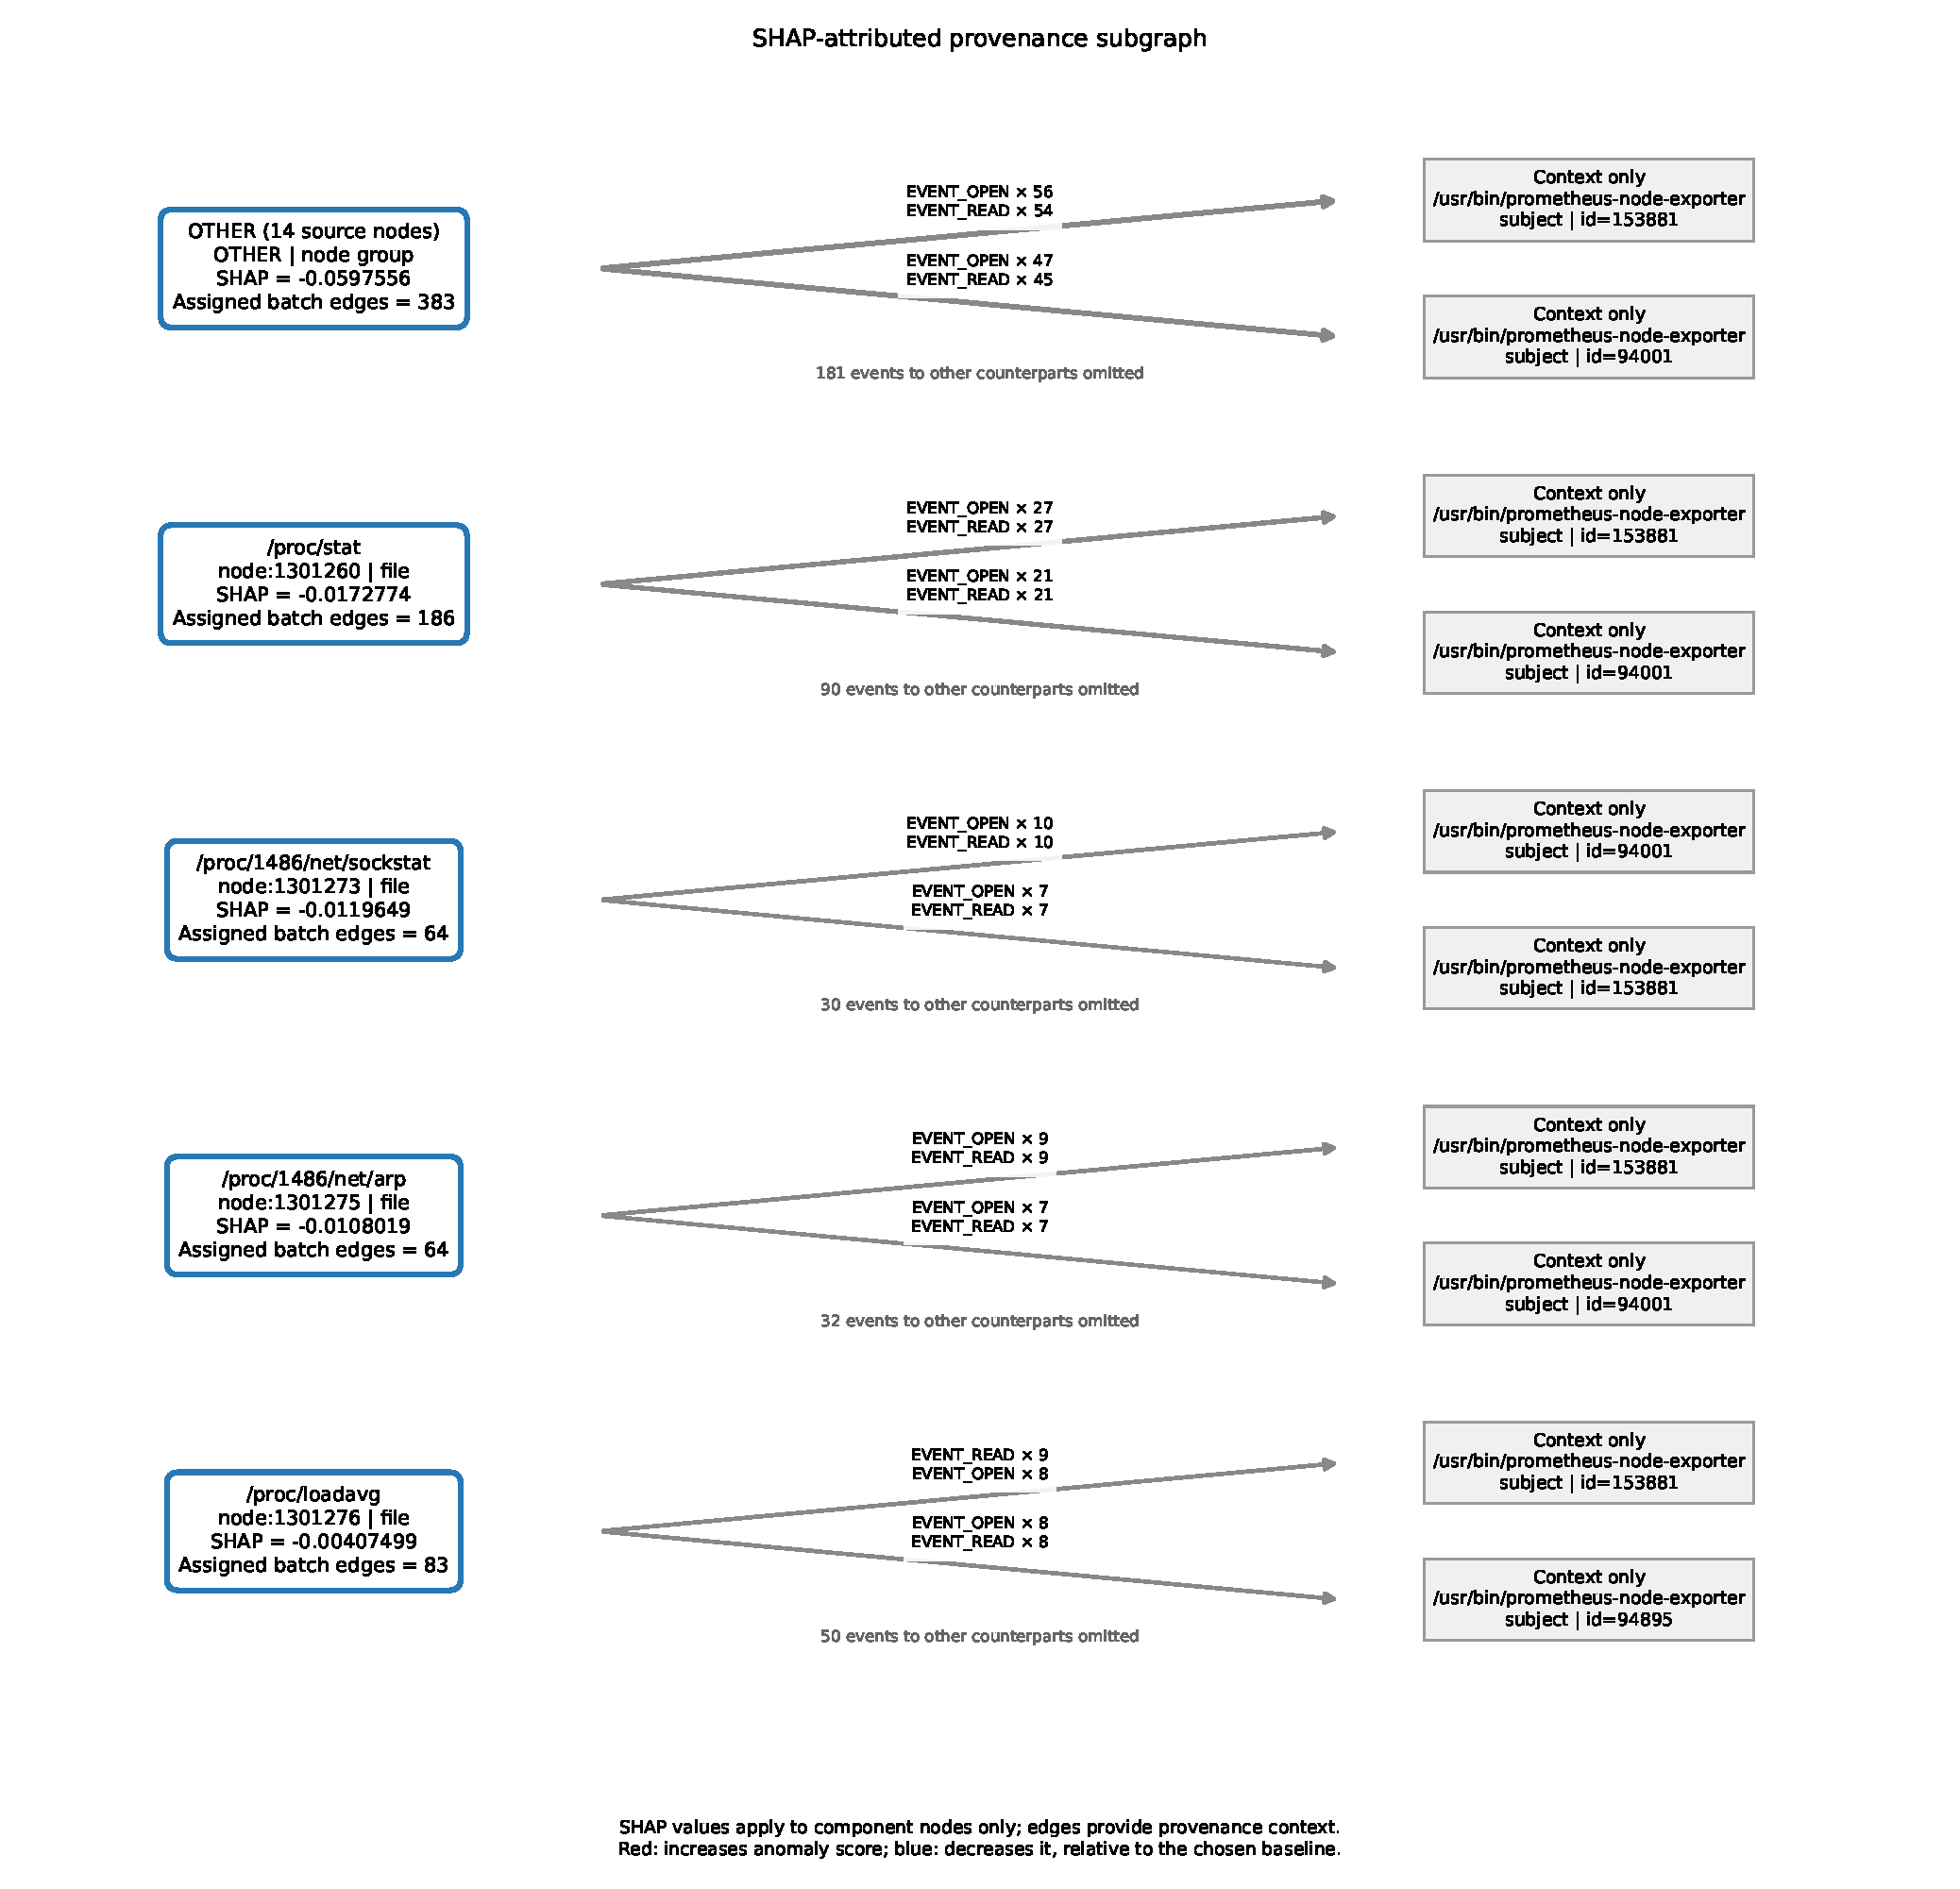
\includegraphics[width=.98\linewidth,height=.80\textheight,keepaspectratio]{figures/initial_provenance.pdf}
\caption{Complete saved initial-validation provenance subgraph, without
cropping. Only the component boxes have SHAP values. Counterparts and arrows
show contextual relationships and event counts, not independent attributions.}
\label{fig:provenance}
\end{figure}

For example, the \path{/proc/stat} component is linked to
\path{/usr/bin/prometheus-node-exporter} subjects through recorded operations.
The source path, counterpart identity and operations together explain what the
numerical group refers to. A raw ID would not communicate that information.
However, the context does not establish that the interaction caused an attack
or that the counterpart has the same SHAP value as the component.

The graph shows the top five components and at most two counterparts per
component. It is a selected view, not the complete temporal graph. Omitted
context counts are indicated by the saved visualizer. The summary table and
JSON keep the full component list. This is why the graph should be read with
the table rather than used as a replacement for all numerical results.

Each view answers a practical question. The bar plot asks which component
values dominate. The waterfall asks how reference and contributions reconstruct
the score. The summary table asks which identity, size and signed value belong
together. The provenance view asks what recorded interactions provide context.
Showing all four makes the output more useful without claiming four independent
forms of validation.

\subsection{Cross-case observations}
The first comparison is between the two high-score cases. Their final scores
are close, but their references and contribution patterns differ. One has a
strong negative hosts-file contribution and a positive whoopsie contribution;
the other has a negative aggregate and seven positive Firefox groups. The
explanation therefore adds information that cannot be recovered from the
scalar ordering alone.

The second comparison is between high and low membership cases. Both have an
endpoint in the exported set, but their scores are far apart. The low case
also exposes the labelled SSH node separately, while the high case places it
inside OTHER. Membership supplies selection context, not a direct rule for
predicting the batch mean or allocating contributions.

Third, the median-reference case has the largest absolute total SHAP change,
but not the largest final score. Attribution magnitude measures a difference
from that case's reference. It is not another anomaly-score scale. Fourth,
every selected case has a negative total contribution, meaning $f(1)<f(0)$
in these five runs. None of these facts makes a component or batch benign.

Fifth, OTHER varies greatly in its contents and role. It includes 14 sources
in initial validation, 220 in the high no-membership case and 966 in the low
membership case. It can dominate the ranking or hide many sources behind a
small value. Interpretation should always include this grouping context.

Finally, mapping and case selection serve different stages of the work. Labels
such as hosts, whoopsie, Firefox, SSH and proc files make a selected explanation
readable. The scan describes many batches and selects coordinates; SHAP explains
the local scalar at those coordinates. Together they provide broad context and
detailed examples, while still stopping short of official detector evaluation.

A practical comparison should therefore begin with the reference and original
score, then inspect the signed components, and finally consult their sizes and
mapped events. For example, the two high scores differ by less than 0.004,
although their neutralized references differ by about 0.243. Their different
total contributions bring them to almost the same final value. Looking only
at the final scores would hide this difference. Looking only at the largest
negative bar would also miss the positive components that partly offset it.
The comparison table and the two bar plots are useful together for this reason.

The group counts also prevent an incorrect reading of OTHER. Its value cannot
be divided equally among its sources to obtain individual SHAP values. In the
saved game, these sources are switched together as one component. Thus the
220-source and 966-source aggregates are different explanation units, even
though both are called OTHER. Their values describe those complete groups
under their own fixed histories. The saved results support comparing their
role in each explanation; they do not support assigning a contribution to
every hidden source without defining and evaluating a different game.

\section{Limitations}
The main limitation is the ORTHRUS reproduction gap. Official pretrained
THEIA\_E5 weights were available, but the original feature and embedding
artifacts associated with those weights were not available in the working
environment. Local THEIA\_E5 artifacts and temporal state had to be reconstructed.
The executed model therefore combined the available parameters with the
locally prepared input representations and temporal context.

This matters because pretrained parameters do not define the whole detector
execution. The features supplied to them and the history available at the
target batch also affect the losses. Using the official model interface and
weight file does not by itself show that the input representations and state
match those used for the published detector. The resulting reproduced behavior
did not match the detector-level baseline reported in the ORTHRUS paper.

The explanations in this project must consequently be attached to the
reproduced instance actually executed. They cannot be claimed to describe the
exact detector used by the ORTHRUS authors. This is not a minor implementation
qualification: it defines the scope of the main scientific claim. A clear
explanation of a reproduced score is still useful, but is a different result
from reproducing published detection performance.

There are two separate questions. \textbf{Explanation fidelity} asks whether
the component contributions account for the selected scalar of the executed
model. The saved full-coalition runs and their residuals provide evidence for
local additive fidelity under the defined perturbation. \textbf{Detector
reproduction} asks whether that executed instance reproduces the original
paper's detector-level behavior. This second condition was not obtained.
A small SHAP residual cannot resolve that mismatch.

The available scan does not supply a substitute detector evaluation. Its means,
percentiles and endpoint memberships characterize batches for selection.
Official evaluation uses a different decision workflow. The high no-membership case and the low membership case are therefore not
assigned batch-level error categories, and detector accuracy is not inferred
from the five examples.
No missing detector metric is filled in with a number derived from membership.

The reconstruction gap also limits comparisons of entity names. A positive
whoopsie value, a negative SSH value or an aggregate Firefox pattern describes
how the reproduced model responds to current features in that case. It is not
a statement that the same entities would have the same values under the exact
published artifacts. Such a transfer would need the corresponding reproduced
detector environment, not only the same explanation code.

Three further limits are practical. First, OTHER reduces granularity. It keeps
all assigned edges in the game, but groups many sources under one value. The
member inside OTHER cannot be given that aggregate's contribution. Changing
the component limit or grouping would ask a different local question, so the
current results should be interpreted with their recorded eight-component
representation.

Second, only five representative batches were deeply explained. They were
chosen to expose useful contrasts in score, membership and local pattern. This
supports a detailed technical case study, not a claim that every test batch has
the same explanation quality or that all possible patterns have been covered.
The full scan gives context for the selection but does not replace missing
explanations of the remaining batches.

Third, the contributions explain model-score changes, not causal attack
behavior. Neutralization keeps topology, targets and past history in place.
A negative value means a decrease relative to that feature reference, not
benign behavior. A positive value is not proof that the entity caused an attack.
These limits remain even when all 256 masks are evaluated. The appropriate
conclusion is local score reconstruction and interpretation for the executed
instance, with its reproduction gap stated openly.

\section{Conclusions}
The project achieved a real integration between ORTHRUS inference and Kernel
SHAP. The final workflow loads a temporal case, builds source-node components,
neutralizes current feature information and returns the mean of the real
per-edge losses. It then maps the resulting contributions to readable entities
and produces numerical and visual explanation records.

The design work was essential to that result. Edge deletion was not used for
the temporal explanation. Current targets and historical context were kept
fixed. Repeated nodes were handled consistently within each role, and every
mask began from the same state immediately before the target batch. These
choices make score comparisons meaningful for the intended current-feature
game instead of mixing them with different model histories.

The complete scan supported representative case selection. Each of the five
final cases used eight components and evaluated all 256 coalitions. Their
reference scores and contributions reconstruct the original scalar with zero
or negligible residual. The bar plots, waterfall, summary table and provenance
view show different useful aspects of those same explanations.

The main observations are concrete. Similar final scores can have very different
component patterns. Exported malicious-node membership does not directly
determine the batch mean. A large total attribution change does not imply a
high original score, and a negative contribution is not a benign label.
Semantic mapping makes these distinctions easier to inspect and discuss.

The main limitation remains the detector reproduction gap. The available
weights, locally reconstructed artifacts and temporal state did not reproduce
the paper's detector-level baseline. The result is an explanation framework
for the model instance actually executed, not a claim of exact reproduction
of the original published detector.

The framework provides faithful component-level explanations of the anomaly
scores generated by the reproduced ORTHRUS instance while preserving the
temporal and structural semantics required by the model.
\end{document}
